\documentclass[10pt]{beamer}

\usepackage[utf8]{inputenc}
\usepackage{tcolorbox}
\usepackage{tikz}
\usepackage{tikz-3dplot}
\usetikzlibrary{intersections,calc,,angles,quotes,through}
\usepackage{amsmath}
\usepackage{graphicx}
\usepackage{cases}
\def \heart {\textcolor{blue}{$\heartsuit$} }
\def \C {\mathcal{C}}
\def \orthog {\underline{\perp}}
\def\arcos{\operatorname{arcos}}
\def \deg {^{\circ}}

\newcommand{\vect}[1] {
  \overrightarrow{#1}}

\tcbset{%
	basic/.style={colframe=black,
		      colback=white,
		      top= 0mm,
		      bottom = 2mm,
		      boxsep=0mm
		      }
}
\tikzset{
    invisible/.style={opacity=0},
    visible on/.style={alt={#1{}{invisible}}},
    alt/.code args={<#1>#2#3}{%
      \alt<#1>{\pgfkeysalso{#2}}{\pgfkeysalso{#3}} % \pgfkeysalso doesn't change the path
    },
  }

    
\begin{document}  
    \beamertemplatenavigationsymbolsempty
    \setlength{\abovedisplayskip}{0pt}
    \setlength{\belowdisplayskip}{0pt}
    \frame{
	  
	  \frametitle{Q3 Septembre 2002.}
	  \renewcommand{\theenumi}{\alph{enumi})}
	  Soit $ABC$ un triangle dont les angles sont aïgus. Le cercle de diamètre $AB$ coupe
	  la hauteur issue de $C$ en des points $X$ et $Y$ ; le cercle de diamètre $AC$ coupe la
	  hauteur issue de $B$ en des points $Z$ et $T$.
	  \begin{enumerate}
	   \item Montrer que $|\vect{AX}|^2=\vect{AB}\cdot\vect{AC}$.
	   \item En déduire que les points $X, Y, Z$ et $T$ sont sur un même cercle, dont on
		 déterminera le centre.
	  \end{enumerate}

	  \vfill
	  
	  \pause
	  % hypothèses et thèse
	  \begin{tcolorbox}[basic] 
	      \begin{columns}[t]
		 
		 \column{.5\textwidth}\centering
		      
		      \underline{Hypothèses} 
		      \begin{itemize}
		      \item $AB,AC$ sont des diamètres,
		      \item $CX,BT$ sont des hauteurs.
		      \end{itemize}

		  
		  \column{.5\textwidth}\centering
		      
		      \underline{Thèse} 
		      \begin{enumerate}
		       \item $|\vect{AX}|^2=\vect{AB}\cdot\vect{AC}$,
		       \item $X,Y,Z,T$ cocycliques.\\ + centre du cercle.
		      \end{enumerate}

		
	      \end{columns}
	  \end{tcolorbox}
    }

    \frame{ 
	  % résolution ex1
	  \begin{columns}[t]
		\column{.5\textwidth}\centering 
		

			\underline{Dessin}\\
				  \vspace{-10mm}
				  \begin{figure}[h]
				  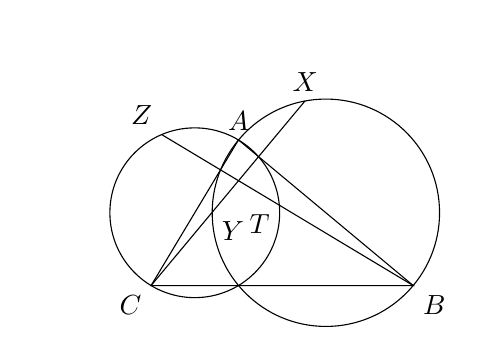
\begin{tikzpicture}[scale=0.74]
			          %projection ($(X)!(B')!(B)$)
			          %nommer chemin 'name path
			          %intersection \path [name intersections={of=d and gb,by=G}];
			          %animation  \draw[visible on=<1>] 
				  %           \draw[visible on=<{2,4}>]
				  %angle arc[radius = 6mm, start angle= 180, end angle= 225] node [below left,pos=0.3]{$\alpha$}
				  %angle \pic [draw,"$\alpha$", angle eccentricity=1.5] {angle = A'--A--B};
				  %perpendiculaire ($(A')!3cm!-90:(A)$)
				  
				   %TRIANGLE ABC
				  \coordinate[label=below left:$C$] (C) at (-1.5,0);
				  \coordinate[label=below right:$B$] (B) at (3,0);
				  \coordinate[label=above:$A$] (A) at (0,2.5);
				  \draw (A) -- (B) -- (C) -- cycle;			
				  %CERCLES
				  \node [draw,name path=C_AB] at ($(A)!0.5!(B)$) [circle through=(A)] {};
				  \node [draw,name path=C_AC] at ($(A)!0.5!(C)$) [circle through=(A)] {};
				  %T,Z
				  \path [name path=BZ] (B) -- +($2*(A)!(B)!(C)-2*(B)$);
				  \path [name intersections={of=BZ and C_AC,name=k}];				
				  \coordinate[label=below left:$T$](T) at (k-1);
				  \coordinate[label= above left:$Z$](Z) at (k-2);
				  \draw (B) -- (Z);
				  %X,Y
				  \path [name path=CY] (C) -- +($2*(A)!(C)!(B)-2*(C)$);
				  \path [name intersections={of=CY and C_AB,name=l}];				
				  \coordinate[label=above:$X$](X) at (l-1);
				  \coordinate[label= below right:$Y$](Y) at (l-2);
				  \draw (C) -- (X);
				  \end{tikzpicture}
				  \end{figure}
			
				  \begin{tcolorbox}[basic] 
				      
				    \smallskip
				    \underline{Hypothèses} 
				    \begin{enumerate}
				    \item $AB,AC$ sont des diamètres,
				    \item $CX,BT$ sont des hauteurs.
				    \end{enumerate}
			            \renewcommand{\theenumi}{\alph{enumi})}		      
				    \underline{Thèse}
				    \begin{enumerate}
				    \item $|\vect{AX}|^2=\vect{AB}\cdot\vect{AC}$,
				    \item $X,Y,Z,T$ cocycliques.\\ + centre du cercle.
				    \end{enumerate}
				    \end{tcolorbox}
		
		
		\column{.5\textwidth}\centering
		
		\underline{Résolution}\\ \flushleft
		\vspace{-3mm}
		\begin{align*}
		|\vect{AX}|^2=& \ (\vect{AB}+\vect{BX})\cdot(\vect{AX}), \\
			     =& \ \vect{AB}\cdot\vect{AX}, \text{ (\textcolor{blue}{1.})} \\
			     =& \ \vect{AB}\cdot(\vect{AC}+\vect{CX}), \\
			     =& \ \vect{AB}\cdot\vect{AC}. \text{ (\textcolor{blue}{2.})}
		\end{align*}
		\hfill $\qed(a)$ \\
		De la même façon, \\ \smallskip
		$|\vect{AY}|^2=\vect{AB}\cdot\vect{AC}$. \\
		\centering\noindent\rule{2cm}{0.4pt}\flushleft
		\vspace{-3mm}
		\begin{align*}
		 |\vect{AZ}|^2=& \ (\vect{AC}+\vect{CZ})\cdot(\vect{AZ}), \\
			     =& \ \vect{AC}\cdot\vect{AZ}, \text{ (\textcolor{blue}{1.})} \\
			     =& \ \vect{AC}\cdot(\vect{AB}+\vect{BZ}), \\
			     =& \ \vect{AC}\cdot\vect{AB}. \text{ (\textcolor{blue}{2.})}
		\end{align*}
		De la même façon, \\ \smallskip
		$|\vect{AT}|^2=\vect{AB}\cdot\vect{AC}$. \\
	        %\hfill $\qed$

   
	   \end{columns}
    
    
    
    }
	\frame{ 
	  % résolution ex1
	  \begin{columns}[t]
		\column{.5\textwidth}\centering 
		

			\underline{Dessin}\\
				  \vspace{-10mm}
				  \begin{figure}[h]
				  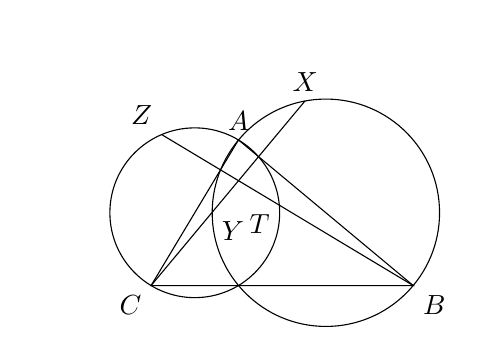
\begin{tikzpicture}[scale=0.74]
			          %projection ($(X)!(B')!(B)$)
			          %nommer chemin 'name path
			          %intersection \path [name intersections={of=d and gb,by=G}];
			          %animation  \draw[visible on=<1>] 
				  %           \draw[visible on=<{2,4}>]
				  %angle arc[radius = 6mm, start angle= 180, end angle= 225] node [below left,pos=0.3]{$\alpha$}
				  %angle \pic [draw,"$\alpha$", angle eccentricity=1.5] {angle = A'--A--B};
				  %perpendiculaire ($(A')!3cm!-90:(A)$)
				  
				   %TRIANGLE ABC
				  \coordinate[label=below left:$C$] (C) at (-1.5,0);
				  \coordinate[label=below right:$B$] (B) at (3,0);
				  \coordinate[label=above:$A$] (A) at (0,2.5);
				  \draw (A) -- (B) -- (C) -- cycle;			
				  %CERCLES
				  \node [draw,name path=C_AB] at ($(A)!0.5!(B)$) [circle through=(A)] {};
				  \node [draw,name path=C_AC] at ($(A)!0.5!(C)$) [circle through=(A)] {};
				  %T,Z
				  \path [name path=BZ] (B) -- +($2*(A)!(B)!(C)-2*(B)$);
				  \path [name intersections={of=BZ and C_AC,name=k}];				
				  \coordinate[label=below left:$T$](T) at (k-1);
				  \coordinate[label= above left:$Z$](Z) at (k-2);
				  \draw (B) -- (Z);
				  %X,Y
				  \path [name path=CY] (C) -- +($2*(A)!(C)!(B)-2*(C)$);
				  \path [name intersections={of=CY and C_AB,name=l}];				
				  \coordinate[label=above:$X$](X) at (l-1);
				  \coordinate[label= below right:$Y$](Y) at (l-2);
				  \draw (C) -- (X);
				  \end{tikzpicture}
				  \end{figure}
			
				  \begin{tcolorbox}[basic] 
				      
				    \smallskip
				    \underline{Hypothèses} 
				    \begin{enumerate}
				    \item $AB,AC$ sont des diamètres,
				    \item $CX,BT$ sont des hauteurs.
				    \end{enumerate}
			            \renewcommand{\theenumi}{\alph{enumi})}		      
				    \underline{Thèse}
				    \begin{enumerate}
				    \item $|\vect{AX}|^2=\vect{AB}\cdot\vect{AC}$,
				    \item $X,Y,Z,T$ cocycliques.\\ + centre du cercle.
				    \end{enumerate}
				    \end{tcolorbox}
		
		
		\column{.5\textwidth}\flushleft
		
		$|\vect{AX}|^2=|\vect{AY}|^2=|\vect{AZ}|^2=|\vect{AT}|^2$. \\ \bigskip
		$\rightarrow X,Y,Z,T$ cocycliques. \\ \medskip Le centre du cercle est $A$.
		
   
	   \end{columns}
    
    
    
    }  
  
\end{document}
